\chapter{Introdução}
\label{chap:intro}

No Brasil, a eletricidade é gerada por hidrelétricas, termoelétricas, parques eólicos e usinas nucleares. Na maioria dos casos, devido a condições geográficas e de segurança, a energia gerada nem sempre é utilizada ou consumida no local de sua geração. Portanto, há a necessidade do uso de linhas de transmissão para transportar energia gerada na fonte geradora para a carga do consumidor \cite{rangel2009sistema}. O mercado consumidor brasileiro é composto de cerca de 47 milhões de unidades. Em termos de linhas de transmissão de energia, são cerca de 98.648,3 km, que devem estar operando 24 horas por dia, 7 dias por semana, 365 dias por ano e em perfeito estado de manutenção, para garantir eletricidade para os consumidores \cite{ons2013dados}

No Brasil, há uma quantidade considerável de linhas de transmissão de alta tensão que já ultrapassaram a vida útil as quais foram destinadas. Com o envelhecimento dos cabos, a inspeção para manutenção preventiva é um fator de extrema relevância para garantir o perfeito funcionamento dos sistemas elétricos. 
De um modo geral, as inspeções nas linhas de transmissão de alta tensão são realizadas regularmente de forma visual, a fim de identificar a necessidade da realização de manutenções preventivas. 
As inspeções buscam verificar a integridade física dos componentes das linhas, em termos de fissuras, corrosão e eventuais danos que venham a prejudicar o fornecimento de energia elétrica. Essas inspeções envolvem a análise da integridade estrutural das torres, da condição dos isoladores, das conexões das linhas de transmissão, dentre outros, a fim de se verificar a existência de eventuais pontos de ruptura. 

Um dos métodos empregados para detecção de pontos quentes nos cabos é o imageamento térmico, que é capaz de identificar uma elevação de temperatura nos cabos, o que é um indício de possíveis pontos de ruptura. A inspeção através de câmera térmica é uma importante ferramenta no campo das inspeções para manutenções preventivas. 
Outros pontos a serem inspecionados envolvem as condições do local onde as torres são instaladas, pois a vegetação e eventuais construções devem ser mantidas a uma distância mínima segura, tal que não ocorra nenhum contato entre quaisquer estruturas e as torres ou cabos de transmissão, evitando assim interferências no funcionamento da linha. 

Além disso, é essencial a garantia de dispor-se de um terreno em condições de trânsito de veículos para o transporte do pessoal de manutenção, transporte de ferramentas, dentre outros fatores. 
Durante vários anos, a inspeção de linhas de transmissão de alta tensão tem sido feita regularmente através de aeronaves tripuladas. As aeronaves executam vôos em baixa altitude e muito próximos das linhas de transmissão conforme mostrado nas  Figuras \ref{img:ihelic} e \ref{img:ihelichuma}.

%---------------picture------------------------------------
\begin{figure}[h!]												
	\centering												
	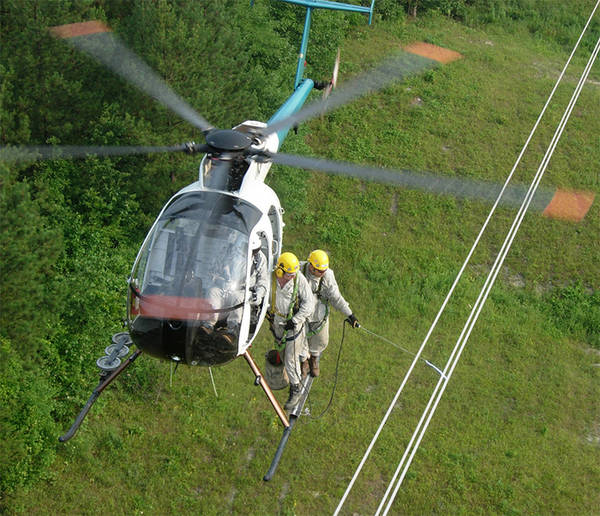
\includegraphics[width=0.6\textwidth]{./insphelic}				
	\caption{Inspeção de linhas de transmissão feita por aeronaves tripuladas.}		
	\label{img:ihelic}												
\end{figure}													
%----------------------------------------------------------
	
%---------------picture------------------------------------
\begin{figure} [h!]												 
	\centering													 
	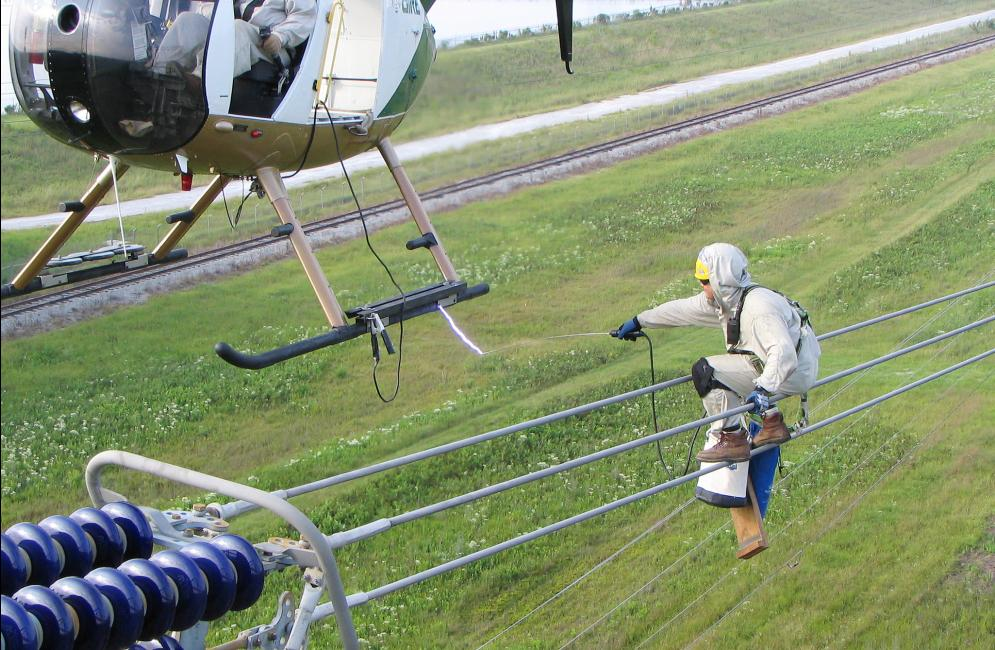
\includegraphics[width=0.6\textwidth]{./insphelichuma}				 
	\caption{Interação humana durante a inspeção de linhas de transmissão.}		
	\label{img:ihelichuma}												 
\end{figure}													 
%----------------------------------------------------------

Em alguns casos, devido às características geográficas da região, condições climáticas e outros fatores que venham a dificultar o sobrevôo, há uma grande exposição dos tripulantes a riscos associados à tarefa. Além dos perigos aos quais os tripulantes são expostos, a inspeção feita com aeronaves tem um custo bastante elevado. Outra forma alternativa de inspeção é o uso de veículos terrestres, porém essa forma é muito limitada, pois boa parte das linhas de transmissão está localizada em áreas de difícil acesso terrestre, muitas vezes restritas pelas características geográficas da região. Além disso, o ângulo de visão é, muitas vezes, desfavorável para a realização da inspeção.

%---------------picture------------------------------------
\begin{figure} [h!]												 
	\centering													 
	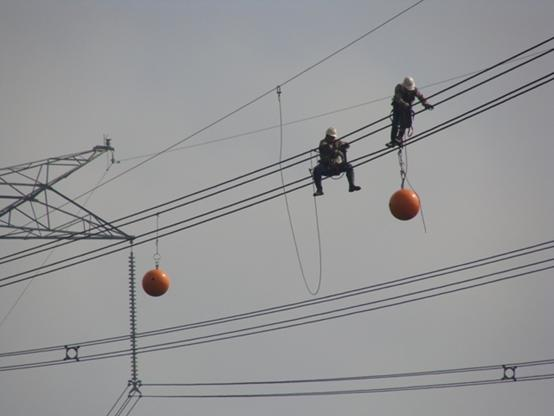
\includegraphics[width=0.6\textwidth]{./insphuma}				 
	\caption{Realização de inspeção em linhas de transmissão através da observação humana.}		
	\label{img:ihuma}												 
\end{figure}													 
%----------------------------------------------------------

Outra maneira de inspecionar as linhas de transmissão é através de eletricistas que literalmente caminham sobre os cabos de linhas de transmissão de alta tensão (Figura \ref{img:ihuma}), realizando inspeção visual e termográfica. Esse tipo de inspeção é lenta e não é viável, tendo em vista que o país possui milhares de quilômetros de linhas de transmissão.

Neste contexto vários robôs de inspeção de linhas de transmissão foram desenvolvidos, porém poucos deles consistiram em projetos de engenharia que sejam aplicáveis no mundo real, além disso a maioria eram robôs tele-operados, ou seja robôs controlados por seres humanos. Um dos pontos diferenciais deste projeto de tese é a proposição de um desenvolvimento de uma navegação autônoma utilizando técnicas de aprendizagem de máquinas até então não utilizadas em robôs de inspeção de linhas de transmissão de alta tensão.

%--------- NEW SECTION ----------------------
\section{Objetivos}
\label{sec:obj}

veja

Nesta se\c{c}\~ao os objetivos principal (tamb\'em
pode-se se utilizar a palavra meta) da monografia de
gradua\c{c}\~ao ou especializa\c{c}\~ao, disserta\c{c}\~ao de
mestrado ou tese de doutorado s\~ao apresentados.


\subsection{Objetivos Específicos}
\label{ssec:objesp}

Nesta se\c{c}\~ao os objetivos espec\'ificos (tamb\'em
pode-se se utilizar a palavra meta) da monografia de
gradua\c{c}\~ao ou especializa\c{c}\~ao, disserta\c{c}\~ao de
mestrado ou tese de doutorado s\~ao apresentados.

%--------- NEW SECTION ----------------------
\section{Justificativa}
\label{sec:justi}

O pesquisador/estudante deve apresentar os aspectos mais
relevantes da pesquisa ressaltando os impactos (e.g. cient\'ifico,
tecnol\'ogico, econ\^omico, social e ambiental) que a pesquisa
causar\'a. Deve-se ter cuidado com a ingenuidade no momento em que
os argumentos forem apresentados.

%--------- NEW SECTION ----------------------
\section{Requisitos do cliente}
\label{sec:reqc}
asjdflkasjdlfjsdlk;f

%--------- NEW SECTION ----------------------
\section{Organização do \thetypework}
\label{section:organizacao}

Este documento apresenta $x$ capítulos e está estruturado da seguinte forma:

\begin{itemize}

  \item \textbf{Capítulo \ref{chap:intro} - Introdução}: Contextualiza o âmbito, no qual a pesquisa proposta está inserida. Apresenta, portanto, a definição do problema, objetivos e justificativas da pesquisa e como este \thetypeworkthree está estruturado;

  \item \textbf{Capítulo \ref{chap:concep} - Nome do capítulo}: XXX;


  \item \textbf{Capítulo \ref{chap:conc} - Conclusão}: Apresenta as conclusóes, contribuições
  e algumas sugestões de atividades de pesquisa a serem desenvolvidas no futuro.

\end{itemize}
